%This research paper---as opposed to a “narrative/composition” paper (e.g., for an English course)---is a written report based on a systematic analysis that you conduct on a topic concerning Complexity Theory in the Social Sciences. Your analysis will apply a selection of concepts, theories, models, or other ideas covered in this course. The actual analysis comes first; the paper comes second, so think of this paper as a “lab report:” you write it up after you have conducted your experiment. Do not begin writing this paper before you have finished (or almost finished) your analysis, otherwise you will likely encounter serious problems. As a general guideline, papers like this are usually 15-20 pages in length. Double-space the entire paper, except the Bibliography.
%
%Use any major citation style (Turabian, MLA, Chicago); just be consistent throughout.
%
%Use any major citation style (Turabian, MLA, Chicago); just be consistent throughout.
\documentclass[pdftex,12pt,oribibl]{llncs}
\usepackage[american]{babel}
\usepackage{wrapfig}
% \newcommand{\x}[1]{ }
% This is where the bibliography stuff needs to happen
%\usepackage[style=apa, backend=biber]{biblatex}
%\DeclareLanguageMapping{english}{american-apa}
\usepackage{biblatex}
\addbibresource{billTolls.bib}
%\addbibresource{Projects-garbageCanCongress.bib}
\usepackage[utf8]{inputenc}
\usepackage{csquotes} % context sensitive quotes ---makes this look good
\usepackage[pdftex]{graphicx}
\usepackage{xfrac}
\usepackage{cleveref}

\begin{document}

%\title{For Whom the Bill Tolls}
%\subtitle{Policy Formation through Simulated Annealing }
\title{A Model of Policy Formation through Simulated Annealing:}
\subtitle{The Impact of Preference Alignment on Productivity and Satisfaction}
\titlerunning{Policy Formation through Simulated Annealing}
\author{Scott Atherley \and Clarence Dillon \and Vince Kane}
\institute{George Mason University\\
\thanks{We wish to thank Maksim Tsvetovat for introducing us to applications of simulated annealing to Organizational Theory and inspiring us to extend and adapt it, and to think about organizations and processes where it seems to fit especially well.  We also thank an anonymous reviewer for helpful feedback provided on a previous draft of this paper.}
\email{\{satherle, cdillon2, vkane2\}@gmu.edu}}

\maketitle

%Cover page: Title, Your Name, ID, Course name, Date, and Abstract ( < 200 words).
%Title: Descriptive, well-focused, and brief. Use a subtitle to provide more information. Some hypothetical examples: “Power Law Analysis of Wealth in Ireland and Peru: A Comparative Analysis”; “Scaling in the International Airline Network“, “Governmental Capacity and Criticality in Domestic Political Instability”; “Comparing Estimates of the Pareto Exponent”. Pick a tentative title first.
%
%Do not settle on a final title until your paper is completely finished.
%

\begin{abstract}
 We are interested in how preference correlations can impact productivity of policy-makers. 
 We apply a simulated annealing process as a model of revising draft legislation in peer and committee reviews before a floor vote determines a congress's approval for a bill.
 We found that having exogenous, common issue priorities has a high impact on productivity but that some structures inhibit productivity, particularly where preferences are uncorrelated.
 
 \textbf{Key words}: simulated annealing, policy formation, organizational theory, preference alignment
\end{abstract}

\section{Introduction}
%(approximately .5 pages) Write this section last!
%A common (bad) idea is to begin by writing this section first—it just doesn’t work because it tends to get too long and disconnected from core results. Introduce the topic of your research and its motivation. Address these questions:
%
%What is the main topic?
%
%Why is it important?
%
%What do some existing works (from readings and your own background bibliographic research) say about this topic?
%
%Conclude this section with a summary paragraph stating (one sentence each):
%the specific topic;
%main hypothesis examined in your analysis;
%approach used for this study;
%major finding. Use boldface each time you use a course term for the first time (e.g., Pareto exponent, criticality, heavy tail, exponential distribution, etc.).

It is a trope of Western democratic ideals that democracy---governance by vote---produces the greatest happiness for its citizenry, or the least unhappiness for the majority.
Our intuition and recent political experience is that diversity and divides in policy preferences can result in legislative deadlock and lower overall satisfaction with legislative outcomes.
Political science often models legislature behaviors backward from voting decisions \parencite{m74, k89}, party influence \parencite{cm93,cm05,a95,k91, k98} and committee dynamics \parencite{sw87, gk89, m04}.
Our research complements other studies by developing a computational model of legislation as a sequential bargaining process.
We considered simulated annealing (SA) to be the non-deterministic optimization method most analogous to the bill revision process; using it to optimize satisfaction within a system of competing legislator preferences. 
The results are broadly applicable to a wide range of policy-making organizations: legislative bodies at the national or local level, regulatory bodies, standards organizations and conference committees, for example.

Our simulation model enables quantitative analysis of the productivity and satisfaction of three typified legislatures: with unified, bi-modal or completely uncorrelated sets of preferences. 
We analyze how the presence of unaffiliated members might moderate partisan deadlock. 
Model results indicate that party partisanship alone does not explain the U.S. Congress's current inability to produce legislation.

\section{Model and Methods}
%(3-4 pages) Write this section third!
%
%This section identifies and defines those concepts, models, theories, or other course ideas and tools that you used in order to carry out your analysis. Which concepts, data, theories, principles or other analytical tools from the course—from lectures or readings—did you use in this study? Which sources?
%
%Which data processing procedures? Which cases or samples? Which time periods (epochs)? Key:reproducibility! I must be able to replicate your findings, based on the information provided in this section.

\subsection{Model Overview}
The model runs 30 times for each of 28 cases---840 times, total---to collect statistically-significant results for each set of key parameters.
We initialize each case by generating a legislature and its internal social network. 
Legislators have preferences on a set of issues; prioritizing issues in some cases.
They take turns sponsoring bills, which get reviewed and revised through two rounds of SA before the entire legislative body votes on the bill.
Our findings reflect data collected about conditions and outcomes for these runs.
We describe the initialization and simulation processes in more detail below.
\footnote{In the interest of brevity, we have omitted some detail descriptions of the initialization and simulation; however, these details,as well as the model itself, may be found in the online supplement at TBD and are referenced where applicable below.}

\subsection{Model Initialization}
The first step in the simulation initializes the model by generating a \texttt{State} object, which contains a realization for the parameters of that run: a heterogeneous set of 100 legislators, each with their own priorities and positions on a set of 75 issues, assigned through a stochastic process. 
The \texttt{State} object then organizes the legislators into a social network making a realistic number of connections between the most similar legislators.

\subsubsection{Initializing the Model Environment}
For our model, we assume that several core issues represent powerful, crystallizing factors that differentiate our simulated parties.
Thus, party ``platforms'' consist of vectors of positions and priorities on a set of issues that includes both \texttt{State\_Priorities} and a random sample of high-priority \texttt{Ideology\_Issues}.
These vectors are used as ``seeds'' for the stochastic generation of individual legislator preferences.

\subsubsection{Legislator Initialization}
Each legislator's issue priorities are assigned with a stochastic preferential attachment method to the seed values provided by the \texttt{State} object.
This generates a power law distribution of priorities for that legislator and provides some correlation in legislator priorities to the extent that seed vectors are correlated through state priorities and party ideology.

We assume that party-affiliated legislators adopt the positions of their party. 
For all other issues (all issues for unaffiliated legislators), the model assigns positions with uniform random probability from the range of allowed position values---$2^4$ for our model.
The end-result of this process is a set of legislator agents with heterogeneous but correlated policy preferences, conditioned by party ideologies and state priorities; with the strength of correlation determined by party-alignment.

\subsubsection{Network Generation}
In the final step of the initialization process, we put legislators into a social network.
The network is generated using both homophily \parencite{msc01, br11} and preferential attachment \parencite{Barabasi1999}, based on preferences assigned in the previous step. 
Preferential attachment is as described in Barabasi and Albert (1999), with $m=5$ new edges selected randomly from a \textit{pdf} distribution of degree in the sub-network of potential allies of each legislator. 
The set of potential allies is selected using an issue-priority weighted likelihood over all issues.
The typical outcome of this procedure is a network among legislator agents with ``small-world'' properties \parencite{Watts1998}, consistent with existing research on social networks in the U.S. Congress \parencite{Granovetter1978} \footnote{We verify ``small-worldness'' of the networks produced by the model using the Humphries and Gurney metrics \parencite{hg08}.}.

\subsection{Simulation Algorithm Overview}
Having defined a population of legislators and their relationship to each-other, we next establish a procedure for legislators to engage in the business of law-making.\footnote{One might argue that this is a departure from realism, as the current Congress does not appear to do this.
However, we are attempting to generalize a model of law-making in legislatures.
Some legislatures do periodically legislate.}
In our model of law-making, the simulation sequentially repeats the following process for 200 proposals (or halts if all issues are passed into law):
\begin{enumerate}
\item Proposal:
\begin{enumerate}
\item A random legislator is chosen to sponsor a bill.
\item The sponsor proposes a draft bill on any issue that has not already been addressed by law. This initial draft reflects the sponsor's position on that issue.
\end{enumerate}
\item Draft circulation among cosponsors:
\begin{enumerate}
\item All legislators connected to the sponsor in the social network are selected as cosponsors.
\item The cosponsors revise the draft using SA; new issues may be added to the bill during the revision process and solutions on existing issues may change.
\end{enumerate}
\item Committee review:
\begin{enumerate}
\item The draft is referred to a committee, reflecting committee agenda-setting powers \parencite{cm93, cm05}.
Legislators for whom the main issue of the bill is a high priority are assigned to the relevant committee.
\item The committee revises the bill by SA; again, new issues may be added and existing solutions changed.
\end{enumerate}
\item Floor vote:
\begin{enumerate}
\item The bill is referred to the floor for a vote.
\item A legislator votes `yes' to a bill when her satisfaction with it is greater than the model parameter \texttt{satisfaction\_threshold}.
\item If the bill passes by simple majority (\textgreater 50\% votes), the bill is made into law; \textit{i.e.}, the solutions addressed by the bill are recorded and the issues may not be revisited for the remainder of the realization.
\end{enumerate}
\end{enumerate}

\subsubsection{Simulated Annealing}
Bill revision is implemented by the Metropolis algorithm for simulated annealing \parencite{mrrt53, kgv}.
Our energy function uses the cumulative dissatisfaction of all reviewers over all dimensions of the bill. 
Increases of $0.1$ in dissatisfaction were accepted with probability \sfrac{1}{2} at the maximum temperature. 
Higher satisfaction energy states are automatically accepted.
See the online appendix for discussion and details about the annealing schedule.

\subsection{Model Calibration}
We calibrated legislators' \textit{satisfaction thresholds}---the point at which they vote ``yes'' on legislation---to achieve a ~4\% pass-rate, comparable to passage rates in the actual U.S. Congress (between 2\% and 7\% in recent history).\footnote{Pass rates are equal to the total number of bills passed in a given Congress divided by the total count of introduced legislation for that Congress. Data to calculate pass rates was collected from Civic Impulse LLC (http://www.govtrack.us).\label{passfn}}

\subsection{Experiments}
Table \ref{params} identifies key parameters used in the model for the suite of experiments.
The simulation program includes a factorial design to run experiments over all combinations of values shown in the table (excepting \texttt{Green\_Fraction} variation when {\texttt{Unaffilitated\_Fraction} = 1.0}, which is a degenerate case), resulting in 28 unique experiments---the cases.
We realized 30 simulations per experiment.

For each realization, we recorded: the number of laws passed, the number of issues addressed by law (i.e. provisions), and legislative body satisfactions over all bills before and after SA revisions. 
To keep the data set manageable, we recorded the run history for only a single realization, as a sample, for each experiment.
Aggregate statistics (averages and standard deviations) were also calculated and recorded for the output metrics of all realizations of an experiment.

\begin{table}
 \caption{Simulation Parameter Space}
 \begin{tabular}{lp{2.25in}c}
 \hline\noalign{\smallskip}
 Parameter & Description & Value [Variation] \\
 \noalign{\smallskip}
 \hline
 \noalign{\smallskip}
 \texttt{Unaffilitated\_Fraction} & Fraction of the legislative population with no ideological party  affiliation. & [0.05, 0.5, 1.0] \\
 \texttt{Green\_Fraction} & Fraction of the party-affiliated population belonging to the \textit{Green} party. Remainder belong to the Yellow party. & [0.5, 0.75, 1.0] \\
 \texttt{Ideology\_Issues} & Ideological platform issues for the parties. & [0, 5] \\
 \texttt{State\_Priorities} & High-priority issues for all legislators, regardless of position on the issue. & [0, 5] \\
 \hline
 \end{tabular}
 \label{params}
\end{table}

\section{Results and Findings}
%(2 pages) Write this section first!
%
%Present your results of analysis in this section. 
Fourteen of the 28 experiment combinations were uniformly unproductive (produced no laws):

\begin{enumerate}
\item All four cases with no party structure,
\item Scenarios with 50\% unaffiliated, 25\% Green, and 25\% Yellow,
\item Scenarios with no external priorities (an additional 5), and
\item One case with 5\% unaffiliated members, 50\% Green members, and no ideology-based priorities.
\end{enumerate}
For the remaining productive cases, Figure \ref{combined} presents run results in each of three aggregate metrics captured for each run (total satisfaction, number of laws passed, and total positive votes), plotted against number of provisions added. 

\begin{figure}[h!]
\centering
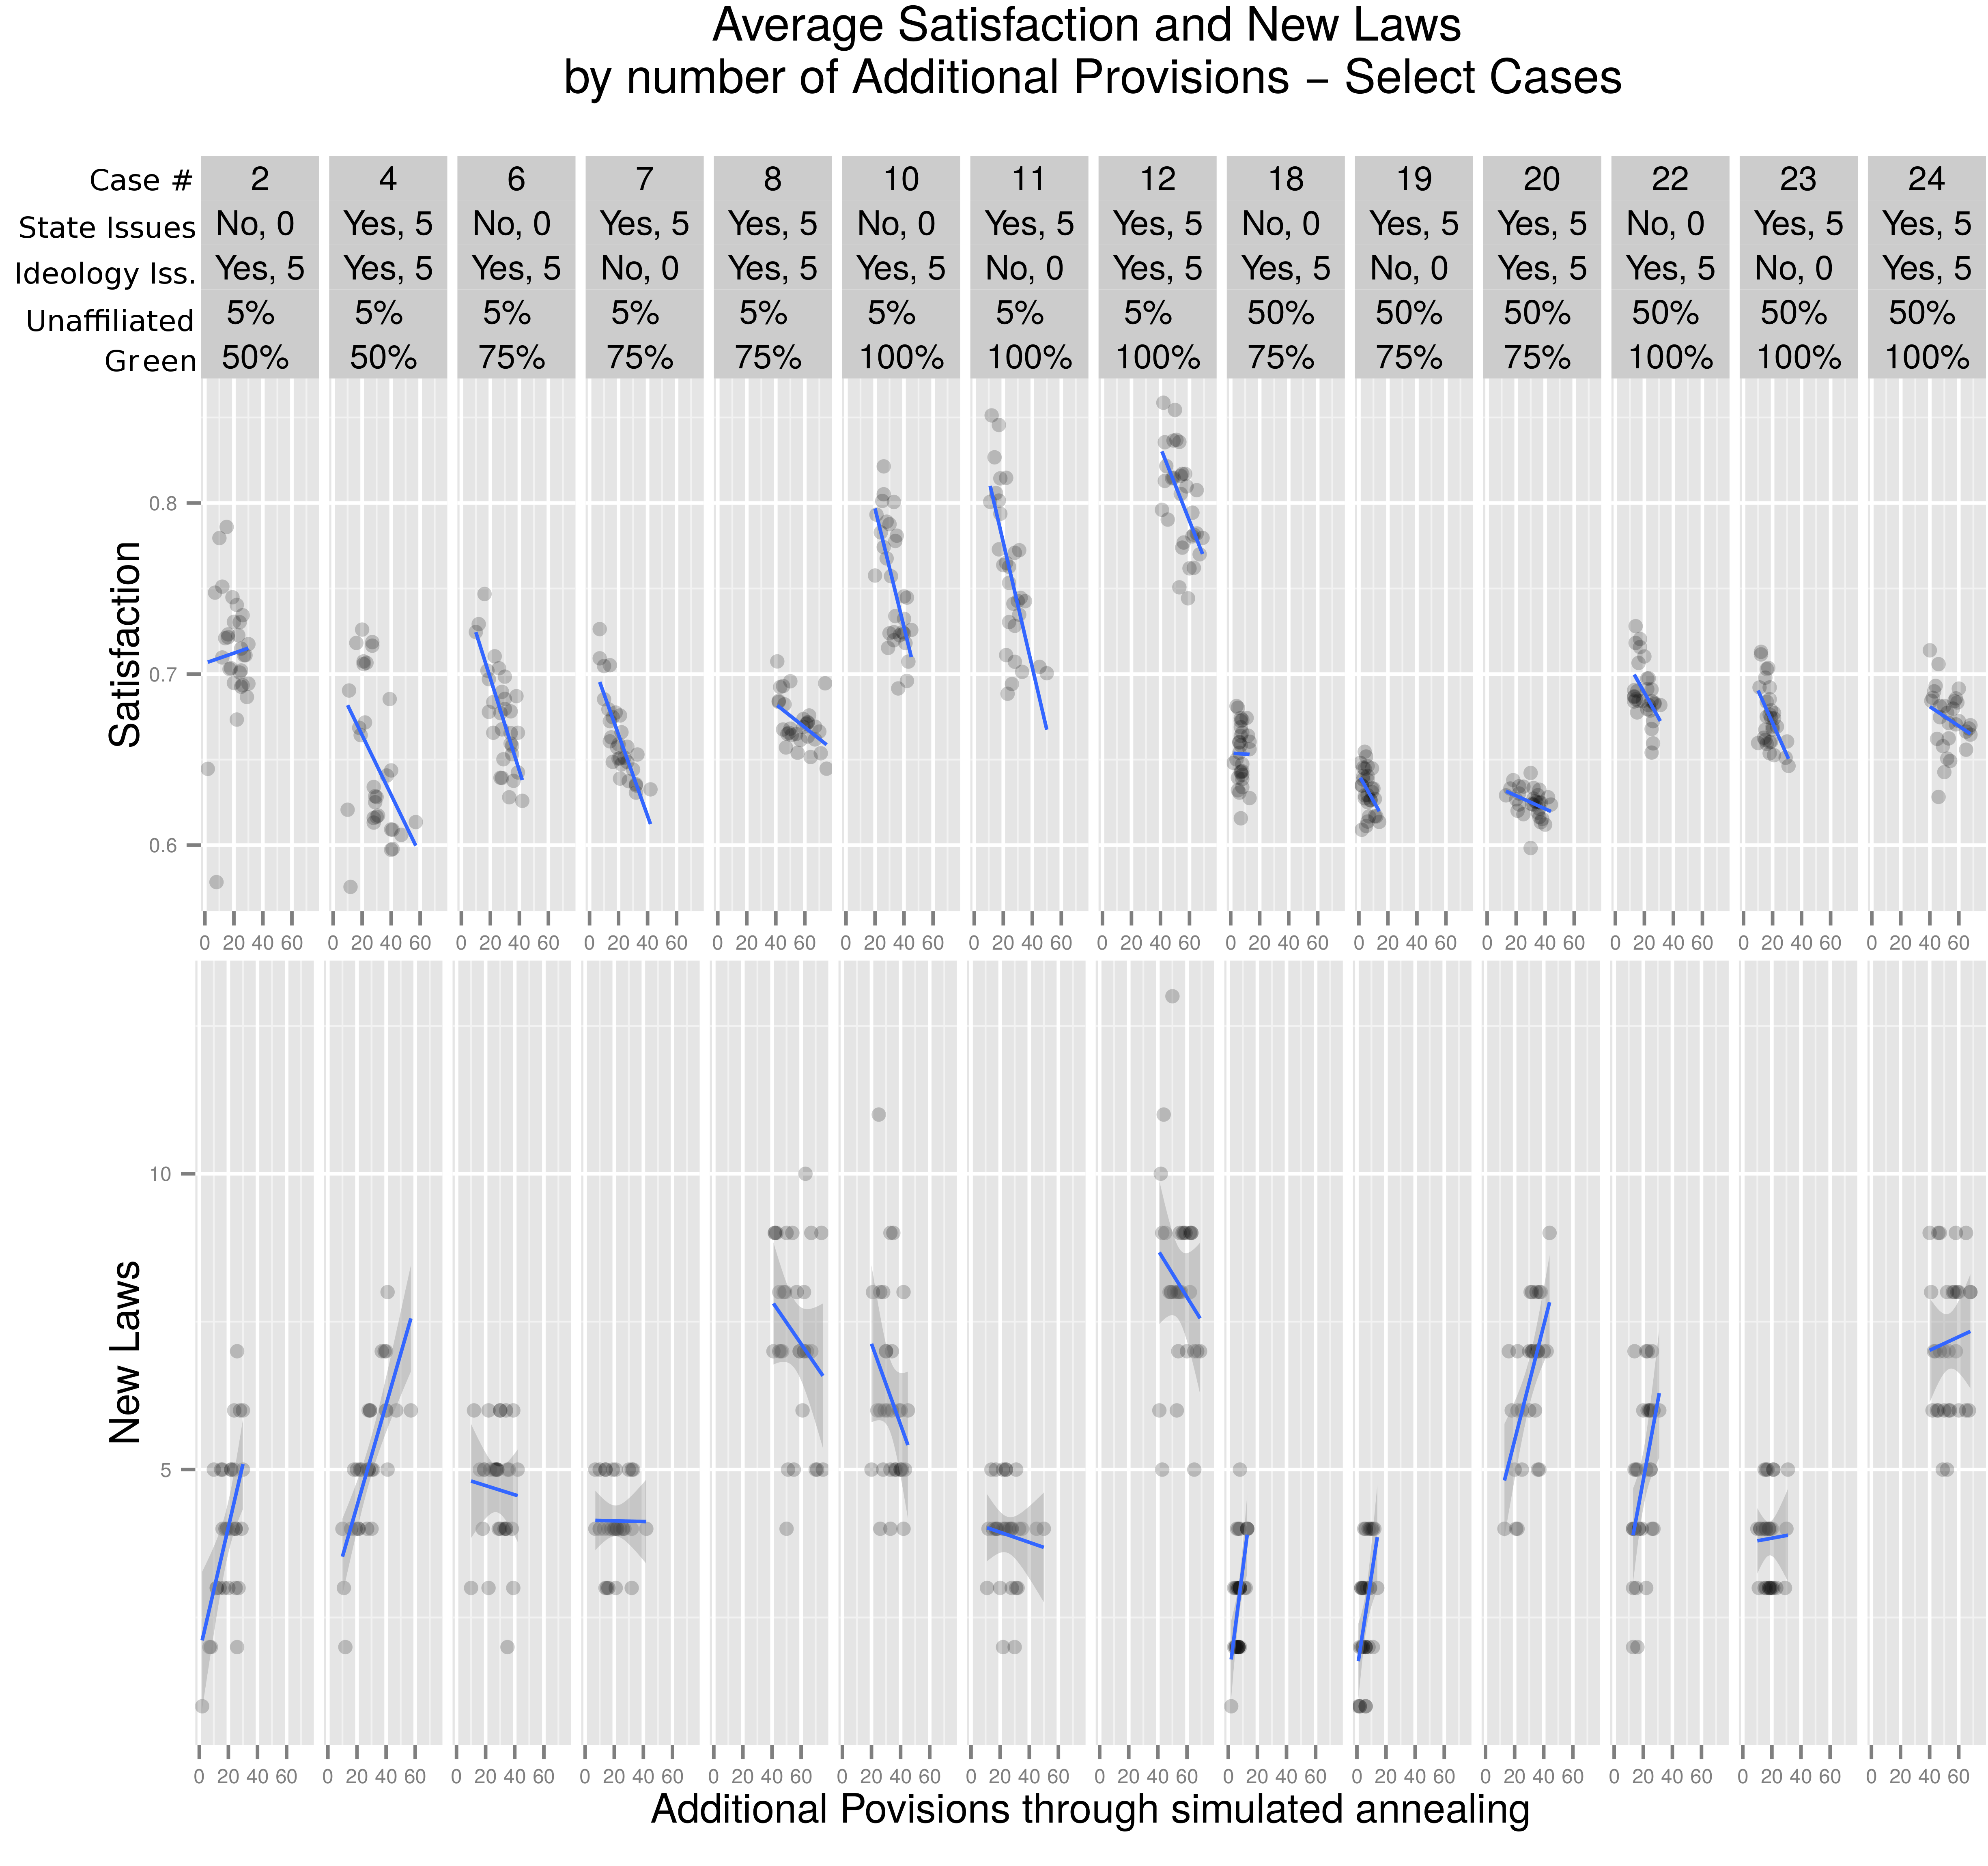
\includegraphics[width=4.75in]{combinedResults.png}
\caption[ ]{Experiment suite results for productive scenarios.  The trend lines indicate a best fit linear correlation to the number of additional provisions.} 
\label{combined}
\end{figure}

%What did your analysis reveal?
%What did the ideas identified in the previous section show you when applied to the topic of your research?
%State your findings using vocabulary learned in the course.
%Imagine making an oral presentation of your main findings or results.
%State your first main finding or result. Then the second, and so on. You may
%want to include graphs, maps, tables, chronologies, diagrams, etc. to support your
%analysis. Label each item.
Interpreting these results, our main findings are:
\begin{enumerate}
\item Higher correlation of preferences results in higher productivity.
\item Higher productivity requires increased provisions.
\item Partisanship is not necessarily an impediment to productivity (see cases 2 and 4).
\item Bipartisan networks (even division of party-affiliated legislators) with more external priorities can be more productive than majorities or super-majorities (with fewer external priorities).  Compare case 4 to cases 11, 18, 19, and 23.
\item Despite higher productivity, overall satisfaction decreases with increased provisions.  Note the prevalence of negative trend lines in the ``Satisfaction'' row of Figure \ref{combined}.
\end{enumerate}

\section{Discussion}
%(3 pages including tables, figures) Write this section second!
%
%This section is entirely based on section 3.
Based on our results and findings, we can generalize about the importance of having external priorities for self-tasking organizations, such as the U.S. Congress, that undertake complex tasks (law generation) requiring group approval.\footnote{Note that production of an academic paper with multiple authors may fit this generalized formulation, as well.}
Having at least some priorities established externally seems to be required for self-tasking organizations to be productive. 
As a rule, the cases with more externally-defined priorities are more productive than the cases with fewer externally-defined priorities. 
We observed very few simulations that passed more laws than the number of externally-defined priorities; and, in no case was it the rule. 
The cases with no externally-defined priorities were consistently unproductive. 
It is tempting to say that this points at the role of leadership---both from within organizations (ideology issues) and from above them (state priorities)---but that will be a question for future research.

Our initial motivation for this research was consideration of the common assertion that a dysfunctional Congress (if measured by ability to pass law) is caused by tensions between the two major political parties in the U.S.
Our results---in particular, findings 3 and 4---do not support the assertion that polarization of preferences alone leads to an unproductive legislature; other factors such as political manipulation are more likely factors.

Finding \#2 demonstrates that higher productivity requires increased provisions.
In a legislative context, these additional provisions, sometimes called, ``riders,'' represent effort diverted to individual interests that are not [necessarily] focused on the task at hand.
These riders represent a the ``cost of doing business''.
Abstracting this from the legislative context, we can generalize that this is higher productivity coming with the cost of lower system efficiency.

Finally, finding \#5---that satisfaction decreases with increasing provisions---captures the social aspects of negotiation and compromise.  
In other words, policy makers are willing to accede adverse positions on their lower-priority issues as a cost of attaining higher satisfaction with the total law, and total satisfaction decreases as these issues are added. 
Conversely, bills start off in a low-satisfaction state and gather provisions as a way of garnering votes.  
In either case, more issues are needed to retain or attain the enough satisfaction to pass new legislation.

\subsection{Implications for future research}
%How would you conduct a follow-up study?
%Would you do things differently?
%How so?
Further research might vary the network-structure generating parameters with finer resolution to discover and understand the tipping points in the outcomes:
How much of a majority is needed before compromise yields dissatisfaction and lower productivity? 
How much leadership intervention (ideology) is required to overcome inherently unproductive structures?  
For completely unaffiliated legislatures, how many state priorities are required to ensure sufficient preference correlation?

We are also interested in understanding the effects of party affiliation on proposals and productivity. This paper reviewed aggregate results from our experiments with the model.
The model could be extended to produce additional data about how much compromise is needed, given the characteristics of a bill's sponsor.
We suspect that the sponsor's peer network, if they are in the minority, may modify an otherwise popular proposal with unpopular issues, such that it fails to garner votes at the committee or floor.
If a bill's sponsor were to intentionally include members from the majority party or, conversely exclude close connections who may be adverse to a proposal, the annealing process might produce more laws.

\section{Summary}
%(<0.5 pages)
%State the main problem or puzzle that motivated this investigation.
%State your major finding
%State your major implication
%\newpage
We modeled policy-making as a simulated annealing algorithm to find solutions in a complex problem space with interdependent constraints.
We chose the U.S. Congress and the American legislative process as a case study, but this research may be applied to other policy-making organizations.
Results indicate that partisanship alone is not necessarily an impediment to productivity, provided that there is sufficient alignment of priorities and preferences.
However, higher productivity comes at the cost of lower satisfaction and system efficiency.
We conclude that simulated annealing is a useful method for computational models of policy-making and that recommend it for other research projects.


\printbibliography
%BIBLIOGRAPHIC REFERENCES (1 PAGE)
%If undecided about style, follow the standard author-year format used in most social
%science publications: e.g., Smith (1990).
%
%Follow standard bibliographic reference format in this section:
%
%Last name, First Name. Year of publication. Title.

%\part{Appendices}
%Supporting documentation.
%Replication-replication-replication!
%
%Any additional supporting document (e.g., source data [BURN A CD FOR THIS], extensive tables, a treaty, Congressional hearings, etc.) or information which is too long to include in the main body of the text because it would distract or interrupt the continuity.
%
%Other guidelines:
%For text, use only 12-point Times font, as in this document. Sansserifed fonts are okay for titles or captions—do not use in text.
%
%Again, double space all text.
%Do not use single spacing.
\end{document}